\documentclass[11pt,a4paper]{article}
\usepackage[margin=2.5cm]{geometry}
\usepackage{amsmath,amssymb,amsthm,mathtools,bm}
\usepackage{graphicx,booktabs,array,multirow}
\usepackage[ruled,vlined,linesnumbered]{algorithm2e}
\usepackage{xcolor}
\usepackage[hidelinks]{hyperref}
\usepackage[capitalise]{cleveref}
\usepackage{caption}
\captionsetup{font=small,labelfont=bf}



\newtheorem{definition}{Definition}
\newtheorem{proposition}{Proposition}
\newtheorem{lemma}{Lemma}
\newtheorem{remark}{Remark}
\newcommand{\R}{\mathbb{R}}
\newcommand{\clamp}{\operatorname{clamp}}
\newcommand{\argmin}{\operatorname*{arg\,min}}
\newcommand{\Sh}{S_h}
\newcommand{\Sv}{S_v}
\newcommand{\NM}{\ensuremath{\,\mathrm{NM}}}

\newcommand{\ROLLval}{0.6}
\newcommand{\Hval}{600}
\newcommand{\Mval}{1}
\newcommand{\MUval}{1.5}
\newcommand{\exN}{15}
\newcommand{\exSh}{7}
\newcommand{\exT}{300}
\newcommand{\exA}{EWG3KP}
\newcommand{\exB}{IBE3247}
\newcommand{\exTf}{216}
\newcommand{\exTmin}{830}
\newcommand{\exDmin}{0.0}
\newcommand{\exSpeedMax}{4.4}
\newcommand{\exMachLo}{0.71}
\newcommand{\exMachHi}{0.82}
\newcommand{\exNsol}{12}
\newcommand{\exGrid}{555}
\newcommand{\exGridMs}{0.6}
\newcommand{\exArcs}{069--221, 338--031}
\newcommand{\exTrk}{230}
\newcommand{\exBest}{\emph{direct TOVRA} (confirmed 9.4\NM) and \emph{direct VEDOD} (confirmed 10.1\NM)}
\newcommand{\exVO}{IBE3247 116$^\circ$, NOZ4381P 37$^\circ$, BAW9522 20$^\circ$}
\newcommand{\spTotal}{99}
\newcommand{\spFeas}{42}
\newcommand{\spSpdN}{12}
\newcommand{\spSpdOk}{0}
\newcommand{\spDctN}{6}
\newcommand{\spDctOk}{2}
\newcommand{\spHdgN}{72}
\newcommand{\spHdgOk}{32}
\newcommand{\spLvlN}{9}
\newcommand{\spLvlOk}{8}
\newcommand{\cpaPairs}{5793}
\newcommand{\cpaConf}{66}
\newcommand{\cpaSits}{123}
\newcommand{\cpaMaxTwenty}{0.70}
\newcommand{\cpaMaxSixty}{4.02}
\newcommand{\hjN}{2422}
\newcommand{\hjAgree}{99.9}
\newcommand{\hjUnav}{18}
\newcommand{\hjFalse}{0}
\newcommand{\hjCons}{46}
\newcommand{\hjMedNear}{0.05}
\newcommand{\hjMeanNear}{0.28}
\newcommand{\hjMirN}{333}
\newcommand{\hjMirOk}{0.60}
\newcommand{\hjMirBad}{2.47}
\newcommand{\stN}{1--30}
\newcommand{\stMatMed}{3}
\newcommand{\stMatMax}{28}
\newcommand{\stDistinct}{10}
\newcommand{\stScn}{5}
\newcommand{\stConf}{64}
\newcommand{\stFut}{39}
\newcommand{\stCur}{25}
\newcommand{\stSolved}{37}
\newcommand{\stSolvedPct}{95}
\newcommand{\stKinds}{heading 28, direct 8, speed 1}
\newcommand{\stConfirmed}{71}
\newcommand{\stSolveMed}{1.1}
\newcommand{\stSolveMax}{12.4}
\newcommand{\stUnsolved}{2}
\newcommand{\stUnsolvedTf}{40}
\newcommand{\stBelowPred}{24}
\newcommand{\stWorstGap}{3.8}
\newcommand{\clBaselineMean}{92.8}
\newcommand{\clBaselineLoss}{2}
\newcommand{\clSolverMean}{97.1}
\newcommand{\clSolverLoss}{0}
\newcommand{\clN}{12}
\newcommand{\clBaseGrades}{left alone 62, other 17, optimal 14, feasible 3}


\title{\textbf{Conflict-free solution sets for en-route air traffic control}\\[4pt]
\large Exact closest-point-of-approach matrices, control-space level sets\\ and Hamilton--Jacobi reachability in a controller training simulator}
\author{Alaa Hamza\\ \small Agadir Area Control Centre}
\date{\small October 2026}

\begin{document}
\maketitle

\begin{abstract}
\noindent
We present the conflict solver of an en-route air traffic control training simulator. Given the predicted
four-dimensional trajectories of every aircraft in a sector, the solver returns, for each predicted loss of
separation, the \emph{set} of clearances --- speed changes, direct routings, delaying vectors with a resume, level
changes, or pairs of them --- that leave the aircraft concerned separated from \emph{every} other aircraft, not only
from the one it conflicts with, ranked in the order a controller would use them. Trajectories are modelled as
piecewise-linear functions of time; on this class the closest point of approach of two aircraft, restricted to the
times at which they are vertically too close, has an exact closed form, computed leg by leg in time linear in the
number of breakpoints. Collecting it over all pairs gives conflict matrices $D^*$ and $T^*$ of the situation. A
clearance is a point $u$ in a control space, and the solution set of an aircraft is the super-level set
$\{u : \Phi(u) \ge \Sh + m\}$ of the function $\Phi(u)$, the closest any other aircraft comes to its trajectory under
$u$. Close in, where turn dynamics matter, a Hamilton--Jacobi reachability table tells whether any turn can still
separate a pair in time. The best solutions are confirmed by running a copy of the full simulation ahead. Traffic
rules of the unit are part of the model: the aircraft maintaining its level, or the first to enter the sector, keeps
priority in it, solutions are taken speed first, then heading, then level, and a level the pilot did not request is
asked first. We give the formulation, the algorithms, their complexity and numerical validation against sampling and
simulation, and evaluate the solver as an autonomous controller on recorded training scenarios.
\end{abstract}

\section{Introduction}

An en-route controller separates aircraft by issuing clearances: a level, a heading, a direct routing to a point
further along the route, or a speed. For each pair of aircraft that will come closer than the separation minima the
controller chooses which aircraft to move and how, under conventions that are as much a part of the job as the
geometry: an aircraft established at its level is not moved out of it if another solution exists; a speed
adjustment is preferred to a vector, a vector to a level change; a level the pilot did not ask for is offered, not
imposed; and a solution must not create a new conflict with a third aircraft.

The simulator this work is part of trains controllers of the Agadir Area Control Centre. It flies every aircraft
with type performance, wind, lateral navigation and simulated pilots who read back clearances or refuse those they
cannot fly. It offers a solo mode, in which a trainee controls a sector alone, and an \emph{AI lab}, in which a
language model controls a sector headlessly and its decisions are evaluated. Both need the same thing: a reference
answer to ``what are the good solutions here?'' --- to show the trainee, to guide the model, and to grade the
decisions of either.

Conflict detection and resolution has a long literature, surveyed by Kuchar and Yang~\cite{kuchar2000}: geometric
methods based on the closest point of approach and velocity obstacles~\cite{fiorini1998,hoekstra2002}, optimisation
over the manoeuvres of several aircraft~\cite{pallottino2002,durand1996}, and reachability analysis by
Hamilton--Jacobi equations~\cite{mitchell2005,tomlin1998}, solved with level-set methods~\cite{osher2003}. We do not claim a new algorithm in each part; the contribution is a coherent, fast and verifiable
pipeline whose output is a \emph{solution set} rather than a single manoeuvre, built on the same trajectory
prediction the radar uses, constrained by operational conventions, and checked against the simulation itself:
\begin{itemize}
\item an exact closest-point-of-approach (CPA) computation for piecewise-linear 4D trajectories with vertical
windows and an RVSM-dependent vertical minimum, and the conflict matrices of a situation (\cref{sec:cpa});
\item velocity obstacles over a heading grid as a fast picture of the free headings (\cref{sec:vo});
\item the solution set as a super-level set of a separation function over a discrete control space, with a cost
encoding the controller's order of preference and the unit's priority and asking rules, and pair combinations
when no single clearance works (\cref{sec:sets});
\item a Hamilton--Jacobi reachability table for close-range pairs, telling whether any turn can still separate them
(\cref{sec:hj});
\item confirmation by simulation, integration in the solo radar and the AI lab, and an evaluation
(\cref{sec:confirm,sec:integration,sec:results}).
\end{itemize}

A design point deserves emphasis. A pairwise method --- including a pairwise Hamilton--Jacobi value function ---
answers ``does this manoeuvre separate $i$ from $j$?'' but not ``does it create a conflict with $k$?''. The solution
set here is defined against \emph{all} predicted trajectories, so a clearance that solves one conflict by creating
another is excluded by construction; the reachability table is used only as a filter on the pair at close range,
where the straight-line prediction is least reliable.

\section{Setting and notation}\label{sec:setting}

\paragraph{Plane and aircraft.} Positions are expressed in a conformal projection of the area in nautical miles,
$x$ east and $y$ north. Aircraft $i$ has position $\bm p_i\in\R^2$, altitude $z_i$ (ft), track $\psi_i$ (degrees
clockwise from north), ground speed $g_i$ (kt, true airspeed composed with the wind), true airspeed $V_i$,
vertical speed $\dot z_i$, its route ahead $R_i=(w_1,w_2,\dots)$ (named points), and the clearances entered in the
system (cleared level, heading, direct, speed). The unit vector of a track $\psi$ is
$\bm e(\psi) = (\sin\psi,\cos\psi)$.

\paragraph{Separation minima.} The horizontal minimum $\Sh$ is a property of the sector (5 or 7\NM\ in the
scenarios used here). The vertical minimum depends on the altitudes:
\begin{equation}\label{eq:sv}
\Sv(z_i,z_j) = \begin{cases}
2000\text{ ft} & \text{if } \min(z_i,z_j)\ge \mathrm{FL}290 \text{ and } \big(\max(z_i,z_j) > \mathrm{FL}410\\
 & \qquad\text{or one aircraft is non-RVSM}\big),\\
1000\text{ ft} & \text{otherwise.}
\end{cases}
\end{equation}
Two aircraft are in \emph{loss of separation} at time $t$ when
$\|\bm p_i(t)-\bm p_j(t)\| < \Sh$ and $|z_i(t)-z_j(t)| < \Sv$. A \emph{predicted conflict} is a predicted loss
within a horizon $H$ ($H = \Hval$\,s in the solver).

\paragraph{Operational conventions.} The unit's conventions, which the solver encodes (\cref{sec:sets}), are:
\begin{enumerate}
\item[(P)] \emph{Priority}: of two aircraft in conflict, one maintaining its level has priority in it over one
climbing or descending; between two level aircraft, the one that entered the sector first keeps its level.
\item[(O)] \emph{Order}: speed adjustment, then a heading (a delaying vector, then resume) or a direct, then a level.
\item[(A)] \emph{Asking}: a level the aircraft did not request is offered first (``able FL370?'') and given only
after an affirmative --- except the level it requested, its flight-plan cruise level, a descent of an arrival, or
an urgent conflict (under 2 minutes) or a loss in progress.
\item[(N)] \emph{No new conflict}: a solution must keep the moved aircraft separated from everyone.
\end{enumerate}

\section{Trajectory model}\label{sec:traj}

\begin{definition}[Piecewise-linear 4D trajectory]
A trajectory over $[0,H]$ is a finite increasing sequence of breakpoints $0=t_0<t_1<\dots<t_K=H$ with positions
$(\bm p_k, z_k)$; between breakpoints, position and altitude are affine in time.
\end{definition}

This is the prediction the radar's medium-term conflict detection makes, written in a form that admits exact
geometry. It is built from three pieces, merged on the union of their breakpoints.

\paragraph{Horizontal path.} The route ahead (or the clearance) gives a polyline $P_0=\bm p_i, P_1, \dots, P_m$,
extended beyond its last point along its last bearing. The aircraft walks it at ground speed $g_0 = g_i$ until the
time $t_s$ of a speed change and at $g_1$ after it; breakpoints are placed at the vertices, at $t_s$ and at $H$.

\paragraph{Clearances as operators.} A clearance $u$ maps the predicted trajectory $X_i$ to $X_i^u$:
\begin{itemize}
\item \emph{Speed} to a Mach number or an indicated airspeed: with $f$ the ratio of the new to the present true
airspeed at the aircraft's level and temperature, the wind is unchanged, so the ground speed changes by the same
amount as the true airspeed:
\begin{equation}
g_1 = \max\!\big(100,\; g_0 + V_i\,(f-1)\big),\qquad t_s = \delta_s = 40\text{ s},
\end{equation}
the time by which most of the change is achieved.
\item \emph{Heading} $\psi'$ for a duration $\tau$, then resume: with the turn $\Delta\psi = |\psi'-\psi_i|$
(wrapped to $[0,180]$), a pilot delay $\delta_p = 6$\,s and a standard-rate turn $\omega=3^\circ/\mathrm{s}$, the turn
is modelled as half on the old and half on the new track:
\begin{equation}
t_\psi = \delta_p + \frac{\Delta\psi}{2\omega},\quad
P_1 = \bm p_i + \tfrac{g_0}{3600}\, t_\psi\, \bm e(\psi_i),\quad
P_2 = P_1 + \tfrac{g_0}{3600}\, \tau\, \bm e(\psi'),
\end{equation}
then direct to the route point after the next one and the route on. Without $\tau$ (an open heading) the
aircraft continues on $\psi'$.
\item \emph{Direct} to a point $w_k$ of the route: the polyline $\bm p_i, w_k, w_{k+1},\dots$.
\item \emph{Level} $L$: the vertical profile below.
\end{itemize}

\paragraph{Turns in progress.} When the aircraft's track differs from the bearing of the first leg --- it has just
passed a point, or a direct was given --- the same half-turn construction is applied: the polyline starts with a
segment of length $\tfrac{g_0}{3600}\,\Delta\psi/(2\omega)$ on the present track. Without it the prediction cuts
the corner, by about half a mile for a $40^\circ$ turn at 450\,kt.

\paragraph{Vertical profile.} With $\Delta z = 100L - z_i$, the rate $r$ is the present vertical speed when it is
in the right direction, above 300\,ft/min, and no new clearance is being given; otherwise the aircraft's own rate
from its performance model: the climb rate available at its level, mass and speed schedule, or its idle descent
rate (times the speedbrake factor 1.5 when it is high on its profile). With a pilot delay $\delta$ for a new level,
\begin{equation}
z(t) = \begin{cases} z_i & t \le \delta\\ z_i + \operatorname{sgn}(\Delta z)\, r\,(t-\delta)/60 & \delta < t < t_L\\ 100L & t\ge t_L\end{cases}
\qquad t_L = \delta + 60\,|\Delta z|/r .
\end{equation}
Since the rate the aircraft will actually fly is uncertain, a candidate level change is checked at two bounds as
well: a \emph{fast} rate, $\max(r, r_{\mathrm{nom}})$ and, in descent, with speedbrakes; and a \emph{slow} rate,
$\min(r, r_{\mathrm{nom}})$, with the nominal $r_{\mathrm{nom}}$ = 1500\,ft/min in climb and 2000 in descent. This is
exact for every rate in between:

\begin{proposition}[Rate bounds]\label{prop:rates}
Let the aircraft cross the level band of another aircraft, entering it after a height $h_a$ and leaving it after
$h_b>h_a$ of climb or descent, at a rate $r\in[r_s,r_f]$. If $h_b/r_f \ge h_a/r_s$ (the windows of the two bounds
overlap), the smallest horizontal distance while vertically too close, over all rates in the interval, is the
smaller of its values at $r_s$ and at $r_f$.
\end{proposition}
\begin{proof}
The horizontal paths do not depend on $r$. At rate $r$ the window is $[h_a/r,\ h_b/r]$ (after the delay), so the union
over $r\in[r_s,r_f]$ is $[h_a/r_f,\ h_b/r_s]$, which equals $[h_a/r_f, h_b/r_f]\cup[h_a/r_s, h_b/r_s]$ when the two
overlap. The minimum of the horizontal distance over a union of windows is the smaller of the minima.
\end{proof}

\noindent For $\Sv = 1000$\,ft the band is 2000\,ft deep and the condition is $r_f/r_s \le 1 + 2000/h_a$: with the
widest bounds used here ($r_f/r_s\approx1.8$) it holds for a band entered within about 2400\,ft of the start of the
climb or descent --- the crossings that matter most, being the soonest. Beyond, the check at the two bounds can miss
an intermediate rate; more rates would close the gap.

\begin{remark}
The model is deliberately the one the controller's tools use: what is checked is the conflict the system predicts.
Its errors --- turn geometry, acceleration, climb performance, wind changes along the path --- are absorbed by a
margin $m$ on the horizontal minimum and, for the best solutions, removed by confirmation in the full simulation
(\cref{sec:confirm}).
\end{remark}

\section{Exact closest point of approach}\label{sec:cpa}

Let $X_i, X_j$ be piecewise-linear trajectories over $[0,H]$ and $U = \{u_0<\dots<u_N\}$ the union of their
breakpoints. On each interval $[u_k,u_{k+1}]$, of length $L_k$, both are affine, hence so is their difference:
\begin{equation}
\bm r(u_k+s) = \bm r_k + \bm v_k s,\qquad \Delta z(u_k+s) = \Delta z_k + w_k s,\qquad s\in[0,L_k],
\end{equation}
with $\bm r=\bm p_j-\bm p_i$, $\Delta z = z_j - z_i$.

\paragraph{Vertical window.} The aircraft are vertically too close on the interval for $s$ in
\begin{equation}
W_k = \{s\in[0,L_k] : |\Delta z_k + w_k s| < \Sv\} =
\begin{cases}
[0,L_k] \text{ if } |\Delta z_k| < \Sv, \text{ else } \emptyset & w_k = 0,\\
\big[\max(0,s_-),\ \min(L_k,s_+)\big] & w_k\ne 0,
\end{cases}
\end{equation}
where $s_\mp$ are the sorted roots $(\pm\Sv - \Delta z_k)/w_k$. Since $\Sv$ depends on the altitudes through
\eqref{eq:sv}, the solver takes on each interval the larger of its values at the two ends, which is conservative.

\begin{lemma}[CPA on a window]\label{lem:cpa}
On a nonempty window $W_k=[a,b]$, the squared distance $\|\bm r_k+\bm v_k s\|^2$ is a convex quadratic in $s$, so
\begin{equation}
d_k = \min_{s\in W_k}\|\bm r_k + \bm v_k s\| = \big\|\bm r_k + \bm v_k\, s_k^*\big\|,\qquad
s_k^* = \clamp\!\Big(-\frac{\bm r_k\cdot\bm v_k}{\|\bm v_k\|^2},\, a,\, b\Big)
\end{equation}
($s_k^*=a$ when $\bm v_k = 0$). The first time in $W_k$ at which the distance falls below $\Sh$ is $a$ if
$\|\bm r_k + \bm v_k a\|<\Sh$, otherwise the smaller root of $\|\bm v_k\|^2 s^2 + 2(\bm r_k\cdot\bm v_k)s +
\|\bm r_k\|^2 - \Sh^2 = 0$ when it lies in $W_k$.
\end{lemma}

\begin{definition}[Pair CPA]
$d^*_{ij} = \min_k d_k$ (with $d_k=+\infty$ on an empty window), attained at $t^*_{ij}$; the pair is in conflict iff
$d^*_{ij} < \Sh$; $t^f_{ij}$ is the first infringement time. The geometry alone (all windows full) gives
$d^{h}_{ij}$, the closest horizontal approach at any level.
\end{definition}

\begin{proposition}[Exactness and cost]
For piecewise-linear trajectories, $d^*_{ij}$ and $t^f_{ij}$ are exact (up to the conservative choice of $\Sv$ per
interval), and their computation takes $O(K_i+K_j)$ operations.
\end{proposition}

\begin{proof}
The minimum over $[0,H]$ restricted to vertical proximity is the minimum over $k$ of the minima over $W_k$; each is
given by \cref{lem:cpa}. The merge of two sorted breakpoint lists and one constant-time step per interval give the
bound.
\end{proof}

\paragraph{Sampling, by contrast.} A detector that evaluates distances every $\Delta$ seconds misses part of the
geometry. On an interval where the window contains the sampling cell around $s^*$, the sampled minimum
$d_\Delta$ satisfies
\begin{equation}\label{eq:sampling}
d^* \le d_\Delta \le \sqrt{d^{*2} + \big(\|\bm v\|\Delta/2\big)^2} \le d^* + \|\bm v\|\,\Delta/2 ,
\end{equation}
because the nearest sample is at most $\Delta/2$ from $s^*$ and $\bm r_k + \bm v_k s^*\perp \bm v_k$ at an interior
minimum. Two aircraft closing at 900\,kt sampled every 20\,s can thus be seen up to 2.5\NM\ further apart than they
will be, and a vertical window shorter than $\Delta$ --- an aircraft climbing through another's level --- can be
missed altogether. \Cref{sec:results} measures both effects.

\paragraph{Conflict matrices.} Over the $n$ aircraft of a situation, the matrices $D^*=(d^*_{ij})$,
$T^*=(t^*_{ij})$ and $C=(d^*_{ij}<\Sh)$ summarise it: the conflicts are the true entries of $C$ ordered by
$t^f$. Their cost is $O(n^2 \bar K)$. An instantaneous variant uses the present velocities: with
$\bm r = \bm p_j - \bm p_i$ and $\bm v = \dot{\bm p}_j - \dot{\bm p}_i$,
\begin{equation}
T^{\mathrm{s}}_{ij} = \clamp\!\Big(-\frac{\bm r\cdot\bm v}{\|\bm v\|^2},0,H\Big),\qquad
D^{\mathrm{s}}_{ij} = \big\|\bm r + \bm v\, T^{\mathrm{s}}_{ij}\big\|,
\end{equation}
vectorised over all pairs at once; it is what the velocity obstacles below are made of.

\section{Velocity obstacles}\label{sec:vo}

For the aircraft $i$ to move and a candidate velocity $\bm u(\psi,g) = g\,\bm e(\psi)$, the relative velocity of
$j$ is $\bm v_r = \dot{\bm p}_j - \bm u$ and the straight-line CPA is that of the previous section. The
\emph{velocity obstacle} of $j$ is
\begin{equation}
\mathrm{VO}_j = \{(\psi,g) : \|\bm r + \bm v_r\,t^*(\psi,g)\| < \Sh\},\qquad
t^* = \clamp\!\big(-\bm r\cdot\bm v_r/\|\bm v_r\|^2, 0, L\big),
\end{equation}
taken over the aircraft $j$ vertically too close to $i$ (or either changing level). In velocity space it is the
classical truncated cone of apex $\dot{\bm p}_j$ and half-angle $\arcsin(\Sh/\|\bm r\|)$; we evaluate it on a
$1^\circ$ heading grid for a few ground speeds. The free set $\mathcal F_i = \complement\bigcup_j \mathrm{VO}_j$ is
reported as arcs of headings. It assumes straight flight and is used as a quick picture --- for the model and for
the trainee (\cref{sec:integration}) --- not as the solver's criterion, which is route-aware.

\section{Solution sets}\label{sec:sets}

\subsection{Control space and separation function}

For an aircraft $i$, the candidate clearances form a finite control set
$\mathcal U_i = \mathcal U^{\mathrm{spd}}_i\cup\mathcal U^{\mathrm{dct}}_i\cup\mathcal U^{\mathrm{hdg}}_i\cup\mathcal U^{\mathrm{lvl}}_i$:
\begin{itemize}
\item speed: from the present Mach $M_0$, $M_0+\delta$ for $\delta\in\{-0.02,\dots,-0.06,+0.01,+0.02,+0.03\}$
within $[0.68,\,\min(0.86, M_{\mathrm{MO}}-0.01)]$; or from the indicated airspeed, $\pm20$ to $\pm50$\,kt within
$[210,340]$;
\item direct: the second to fourth points of the route ahead;
\item heading: $\psi_i+\Delta\psi$, $\Delta\psi\in\{\pm10,\pm20,\pm30,\pm45,\pm60,\pm90\}$, for
$\tau\in\{120,240,360\}$\,s, then resume;
\item level: $\pm1000$ to $\pm4000$\,ft from the cleared level, of the aircraft's direction (semicircular rule)
unless an arrival descends, under its ceiling.
\end{itemize}
Each candidate is first submitted to the simulated pilot's own check $\mathcal P_i$ (performance at its level and
weight, weather, RVSM approval): a clearance the pilot would refuse is not a solution.

\begin{definition}[Separation function]
For $u\in\mathcal U_i$, with $X_i^u$ the trajectory under $u$ and $X_j$ the predicted trajectories of the others,
\begin{equation}
\Phi_i(u) = \min_{j\ne i} d^*\big(X_i^u, X_j\big).
\end{equation}
\end{definition}

\begin{definition}[Solution set]
With a margin $m$ ($m=\Mval$\NM),
\begin{equation}
\mathcal S_i = \{u\in\mathcal U_i\cap\mathcal P_i : \Phi_i(u)\ge \Sh + m\}.
\end{equation}
\end{definition}

$\mathcal S_i$ is the super-level set $\{\Phi_i\ge \Sh+m\}$ of $\Phi_i$ restricted to the flyable controls: the
level-set view of the problem. Its boundary $\{\Phi_i = \Sh+m\}$ separates, in the plane of a delaying vector's
heading change and duration, the vectors that work from those that do not (\cref{fig:sets}). Because $\Phi_i$ takes
the minimum over \emph{all} other aircraft, requirement (N) holds by construction:

\begin{proposition}[No new conflict]
If $u\in\mathcal S_i$ and the other aircraft follow their predicted trajectories, aircraft $i$ under $u$ has no
predicted conflict with any aircraft over $[0,H]$, with margin $m$.
\end{proposition}

Evaluating $\Phi_i(u)$ costs $O\big((n-1)\bar K\big)$ by \cref{lem:cpa}; with early exit as soon as one pair falls
under $\Sh+m$, rejected candidates are cheap.

\subsection{Costs, priority and the asking rule}

The controller's order (O) is encoded in a cost whose kind offsets dominate the magnitude terms:
\begin{equation}
J(u) = \begin{cases}
0.08\,|\delta|/0.01 & \text{speed (per 0.01 Mach or 10 kt)}\\
1.0 + 0.05\,k & \text{direct to the $(k{+}1)$-th point ahead}\\
1.2 + 0.06\,|\Delta\psi|/10 + 0.05\,\tau/120 & \text{delaying vector}\\
3.0 + 0.15\,|\Delta L|/1000\text{ ft} + 0.5\,\mathbb 1_{\mathrm{ask}} & \text{level}
\end{cases}
\;+\; 5\cdot\mathbb 1_{\mathrm{prio}} ,
\end{equation}
with $\mathbb 1_{\mathrm{prio}}=1$ when $i$ has priority. Priority (P) is decided per pair: the aircraft changing level moves if the other is level; between two level
aircraft, the later to enter the sector moves (a tie within 5\,s gives no priority). Moving the aircraft with
priority costs 5, more than any single clearance of the other, so it is proposed only when nothing else works. The
asking rule (A) adds 0.5 to a level the pilot did not request and marks it \emph{ask first}. The \emph{optimal} set
is
\begin{equation}
\mathcal O = \{u\in\mathcal S : \mathrm{kind}(u)=\mathrm{kind}(u^\star),\ J(u)\le J(u^\star)+\varepsilon\},
\qquad u^\star=\argmin_{\mathcal S}J,\ \varepsilon = 0.3 .
\end{equation}
Reporting a set rather than $u^\star$ alone matters for grading: two directs a few miles apart, or a vector of
$20^\circ$ or $30^\circ$, are equally good answers.

\subsection{Pairs of clearances}

When neither aircraft of the conflict has a single solution, the solver keeps, for each, the six candidates that
increase most its distance to the other, and searches the $6\times6$ pairs $(u_i,u_j)$ such that
$\Phi_i(u_i)\ge \Sh+m$ given $X_j^{u_j}$ and $\Phi_j(u_j)\ge \Sh+m$ given $X_i^{u_i}$, at cost
$J(u_i)+J(u_j)+1$. If none exists the conflict is reported as needing a combination or action on third traffic.

\begin{algorithm}[t]
\caption{Solution sets of a situation}\label{alg:solve}
\KwIn{world $w$, horizon $H$, margin $m$, rollouts $k$}
$X \gets$ predicted trajectories of all active aircraft\;
$\mathcal C \gets$ conflicts of $C(X)$ involving an assumed aircraft, ordered by $t^f$\;
\ForEach{$(a,b)\in\mathcal C$}{
  decide the aircraft to move by (P); order $=(\text{mover}, \text{other})$\;
  \ForEach{$i$ in order}{
    \lIf{$t^f\le T_{\mathrm{HJ}}$, both level, and $V_{\mathrm{HJ}}(i,\cdot)\le \mu$}{drop heading and direct candidates}
    \ForEach{$u\in\mathcal U_i\cap\mathcal P_i$}{
      build $X_i^u$; $\Phi\gets\min_{j\ne i} d^*(X_i^u,X_j)$\;
      \lIf{$\Phi\ge \Sh+m$}{add $u$ to $\mathcal S$ with cost $J(u)$}
    }
  }
  \lIf{$\mathcal S=\emptyset$}{search pairs of the best partial moves}
  sort $\mathcal S$ by $J$; confirm by rollout the first ones until $k$ are confirmed (at most $k+4$)\;
  drop refuted solutions; $\mathcal O\gets$ optimal set\;
}
\end{algorithm}

\section{Close range: Hamilton--Jacobi reachability}\label{sec:hj}

The straight-line and route-aware predictions treat a turn as an instantaneous change of track after a delay. Close
in, the turn itself decides the outcome. For a pair, we ask: \emph{can the moved aircraft, by turning alone at up to
a standard rate, still avoid the other, which flies straight on?}

\paragraph{Relative dynamics.} In the frame of the moved aircraft (1), with $x$ along its track and $y$ to its right,
let $(x,y)$ be the position of the other (2) and $\theta = \psi_2-\psi_1$ the track difference (clockwise, as tracks are). With speeds
$v_1,v_2$ and the turn rate $u$ of aircraft 1, $|u|\le\omega$:
\begin{equation}\label{eq:rel}
\dot x = -v_1 + v_2\cos\theta + u\,y,\qquad
\dot y = v_2\sin\theta - u\,x,\qquad
\dot\theta = -u .
\end{equation}
The target is the loss of separation, $\mathcal T = \{l(\bm\xi)\le 0\}$ with $l = \sqrt{x^2+y^2}-\Sh$ and
$\bm\xi=(x,y,\theta)$.

\paragraph{Backward reachable tube.} The set of states from which a loss cannot be avoided within $T$ whatever the
turn is $\{V(\cdot,T)\le 0\}$, where $V$ is the viscosity solution~\cite{crandall1983} of the Hamilton--Jacobi--Isaacs variational
inequality
\begin{equation}\label{eq:hji}
\frac{\partial V}{\partial \sigma} = \min\Big(0,\ \mathcal H\big(\bm\xi,\nabla V\big)\Big),\qquad V(\bm\xi,0) = l(\bm\xi),
\end{equation}
in the backward time $\sigma$, the $\min(0,\cdot)$ freezing the tube: once unavoidable, unavoidable. The aircraft
maximises the distance, so
\begin{equation}
\mathcal H(\bm\xi,\bm q) = \max_{|u|\le\omega} \bm q\cdot\bm f(\bm\xi,u)
= q_1(-v_1+v_2\cos\theta) + q_2 v_2\sin\theta + \omega\,\big|q_1 y - q_2 x - q_3\big|,
\end{equation}
since $\bm q\cdot\bm f$ is affine in $u$ with slope $q_1y-q_2x-q_3$. The optimal turn is bang-bang,
$u^\star = \omega\,\operatorname{sgn}(q_1y-q_2x-q_3)$, and gives the direction of escape.

\paragraph{Numerical scheme.} \Cref{eq:hji} is solved on a $101\times101\times60$ grid (the formulation and scheme follow~\cite{mitchell2005,osher2003}) over
$[-45,45]^2\NM\times[0,2\pi)$, periodic in $\theta$, by a first-order Lax--Friedrichs scheme with central
differences $\bar q$ and \emph{local} dissipation coefficients
\begin{equation}
\alpha_x = |-v_1+v_2\cos\theta| + \omega|y|,\quad \alpha_y = v_2|\sin\theta| + \omega|x|,\quad \alpha_\theta = \omega,
\end{equation}
\begin{equation}
V^{n+1} = V^n + \Delta\sigma\,\min\!\Big(0,\ \mathcal H(\bm\xi,\bar{\bm q}) + \tfrac12\textstyle\sum_d \alpha_d\,(q_d^+-q_d^-)\Big),
\end{equation}
with the time step set by a CFL number of 0.8:
$\Delta\sigma = 0.8/\big(\bar\alpha_x/\Delta x+\bar\alpha_y/\Delta y+\alpha_\theta/\Delta\theta\big)$. A global
dissipation coefficient, set by the turning term at the edge of the grid ($\omega L$), smeared the solution over
several miles; the local one does not. The horizon is $T=300$\,s, $v_1 = 450$\,kt, and one table is computed per
speed ratio $v_2/v_1\in\{0.8,0.9,1.0,1.1,1.2\}$ and per minimum $\Sh$, once (about a minute each), and stored;
a lookup is a trilinear interpolation.

\paragraph{Use.} For a conflict with $t^f\le T$ in which both aircraft are level, the solver looks up
$V$ at the pair's relative state; if $V\le\mu$ for the aircraft to move, no turn of that aircraft separates the
pair in time and its heading and direct candidates are dropped (only speed --- rarely enough at that range --- or a
level remain). The threshold $\mu=\MUval$\NM\ absorbs the optimism of the first-order scheme measured in
\cref{sec:results}.

\section{Confirmation by simulation}\label{sec:confirm}

The candidates are ranked on the trajectory model; the best are then confirmed on the simulator itself. The world
is copied (aircraft, performance and weight, wind, weather, entries, pilots), the clearance is entered as a
controller would --- refused if the simulated pilot would refuse it --- and the copy is advanced by one-second steps
over $H$, a delaying vector being resumed after $\tau$. Every two seconds, the distance of each moved aircraft to
every aircraft vertically too close to it is recorded; the solution is \emph{confirmed} when the minimum stays at or
above $\Sh$, and refuted otherwise. The rollout costs $\ROLLval$\,s per solution for a ten-minute horizon; the
solver confirms the cheapest solutions until $k$ ($k=2$ by default) are confirmed, trying at most $k+4$.
Refuted solutions are removed from the set.

\section{Integration in the simulator}\label{sec:integration}

\paragraph{Solo radar.} A \emph{Solver} panel lists, for each predicted conflict involving one of the trainee's
aircraft, the conflict ($d^*$ and time to first infringement), the priority reason, and the solutions in cost order
with their kind, the predicted or confirmed distance, and \emph{ask first} or \emph{priority} marks. \emph{Apply}
enters the clearance in the label exactly as the trainee would; a delaying vector leaves a resume reminder with a
countdown. The panel is refreshed every five simulated seconds or when an entry changes.

\paragraph{AI lab.} The solver is used in three ways. (i) As a controller of its own: a built-in agent assumes and
transfers aircraft, answers requests, and applies the optimal solution of each conflict, giving a reference score
for each scenario. (ii) As hints in the observation given to a language model: each conflict line ends with the
solver's best and other options. (iii) As a grader: each decision of any agent on a conflict is classified as
\emph{optimal} (in $\mathcal O$), \emph{feasible} (in $\mathcal S\setminus\mathcal O$), \emph{other}, or
\emph{left alone}, and the labels of the experience dataset carry a reward of $+2$, $+1$ and $-1$ for the first
three. The model can also query the solver (\texttt{solve}) and the velocity obstacles (\texttt{headings}).

\section{Results}\label{sec:results}
All experiments use the simulator's own scenarios of the Agadir airspace (Moroccan upper airspace, four sectors) and
its own code; the figures are drawn from simulated situations.

\subsection{A worked example}

\Cref{fig:traj} shows the West North sector of scenario \emph{p02} at T+\exT\,s, with \exN\ aircraft on the picture and
$\Sh=\exSh\NM$. Two aircraft at FL350, \exA\ and \exB, are on routes merging at a common point; the solver predicts a
first infringement in \exTf\,s and, on a longer horizon, a closest approach of \exDmin\NM\ at \exTmin\,s: without
action they would be in trail at the same point and level. They entered the sector together, so neither has priority.

\begin{figure}[t]
\centering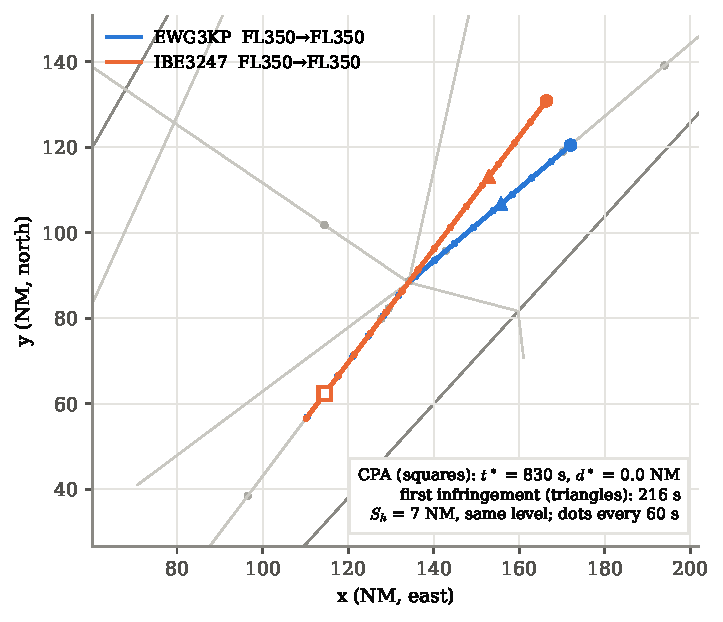
\includegraphics[width=0.72\linewidth]{figs/f1_trajectories.pdf}
\caption{Predicted piecewise-linear trajectories of a situation (grey), the conflicting pair in colour. Squares: the
closest point of approach; triangles: the first infringement of the minima, both exact (\cref{lem:cpa}).}
\label{fig:traj}
\end{figure}

\paragraph{Velocity obstacles.} \Cref{fig:vo} gives the headings of \exA\ that bring it within $\Sh$ of another aircraft
flying straight on (at its present ground speed): \exVO. Its present track \exTrk\ lies inside the obstacle of
\exB; the free arcs are \exArcs.

\begin{figure}[t]
\centering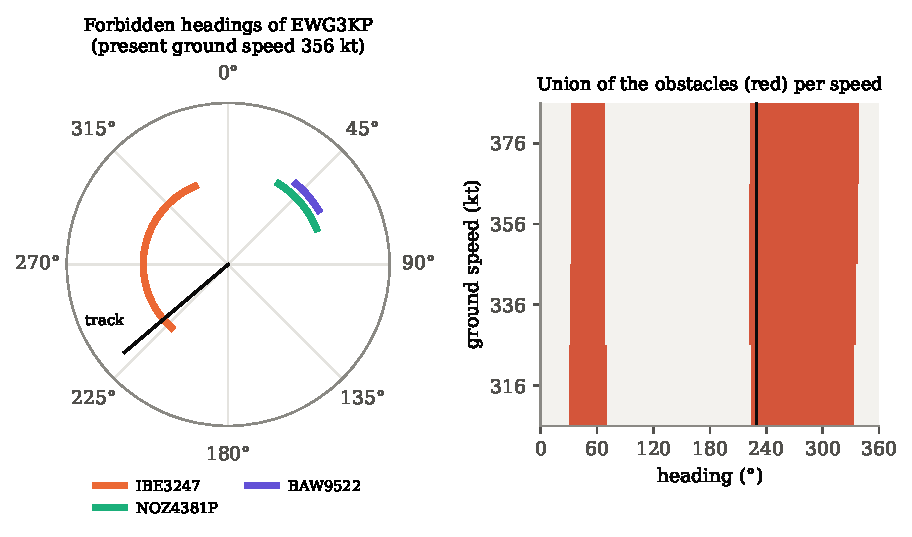
\includegraphics[width=0.95\linewidth]{figs/f3_vo.pdf}
\caption{Velocity obstacles of the aircraft to move. Left: forbidden headings per other aircraft (arcs) and the
present track. Right: their union over heading and ground speed.}
\label{fig:vo}
\end{figure}

\paragraph{Solution set.} \Cref{fig:sets} shows $\Phi$ over the plane of a delaying vector (heading change and
duration, then resume), sampled on \exGrid\ controls (\exGridMs\,ms each), and over speed alone. Speed cannot solve
this conflict: over Mach \exMachLo--\exMachHi\ the closest approach to anyone stays under \exSpeedMax\NM. The
super-level set $\{\Phi\ge\Sh+m\}$ is the region of left turns of $20^\circ$ and more; right turns bring the aircraft
towards other traffic. The solver returns \exNsol\ solutions; the optimal set is \exBest, both shortening the route
(direct before vector in the order of preference).

\begin{figure}[t]
\centering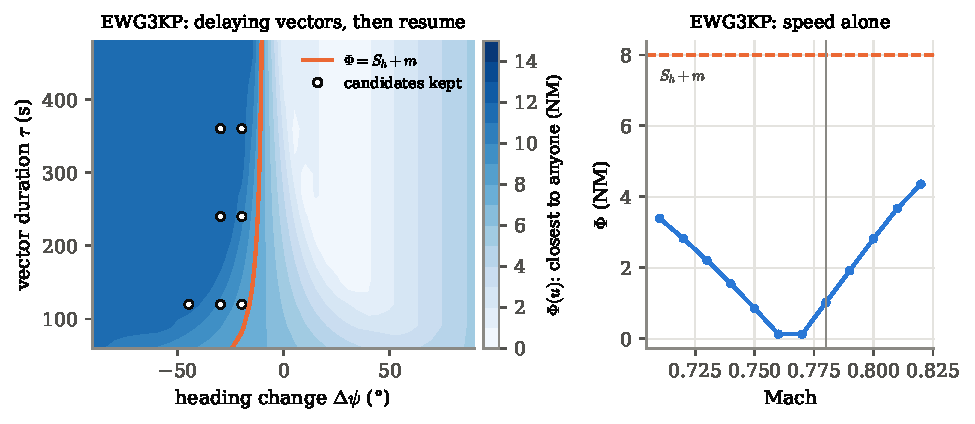
\includegraphics[width=\linewidth]{figs/f4_solutionset.pdf}
\caption{The separation function $\Phi$ of the aircraft to move. Left: over delaying vectors; the solution set is the
region beyond the orange level line $\Phi=\Sh+m$; circles: the vectors of the solver's control grid kept as
solutions. Right: over speed alone (all below $\Sh+m$).}
\label{fig:sets}
\end{figure}

\subsection{Exact CPA against sampling}

Over \cpaSits\ situations taken every two minutes in ten scenarios (aircraft not controlled), the \cpaPairs\ pairs
coming within 60\NM\ of each other were evaluated exactly and by sampling the same trajectories every $\Delta$
seconds (\cref{tab:sampling}, \cref{fig:sampling}). The error grows with $\Delta$ as \eqref{eq:sampling} predicts: up
to \cpaMaxTwenty\NM\ at 20\,s, the step of the radar's medium-term detection, and \cpaMaxSixty\NM\ at 60\,s. In
these situations no vertical window was lost and no conflict missed at any step: the main effect of sampling is the
distance it reports, which decides whether a marginal conflict is shown and whether a clearance clears it by the
margin. The windows a sampling can lose are short ones --- a climb or descent crossing another level --- which these
uncontrolled situations contain few of.

\begin{table}[t]
\centering\small
\caption{Sampled minimum minus exact minimum distance (NM) while vertically too close, over the pairs within 60\NM.
\emph{Window lost}: the sampling never sees the pair vertically too close although it is; \emph{conflicts missed}:
exact conflicts (of \cpaConf) the sampled distance does not show.}
\label{tab:sampling}
\begin{tabular}{rrrrrr}
\toprule
$\Delta$ (s) & median & 95th pct. & max & window lost & conflicts missed\\
\midrule
1 & 0.00 & 0.00 & 0.04 & 0 & 0 \\
5 & 0.00 & 0.01 & 0.21 & 0 & 0 \\
10 & 0.00 & 0.03 & 0.35 & 0 & 0 \\
20 & 0.00 & 0.06 & 0.70 & 0 & 0 \\
30 & 0.00 & 0.29 & 1.95 & 0 & 0 \\
60 & 0.00 & 1.02 & 4.02 & 0 & 0 \\
\bottomrule

\end{tabular}
\end{table}

\begin{figure}[t]
\centering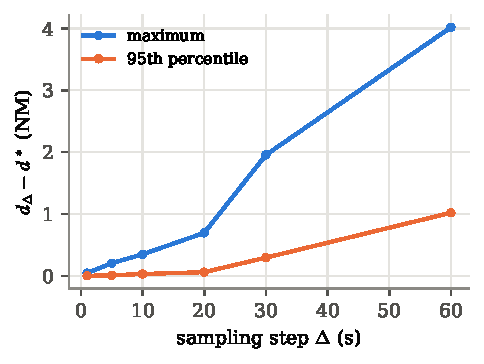
\includegraphics[width=0.48\linewidth]{figs/f2_sampling.pdf}
\caption{Error of a sampled minimum distance against the exact CPA.}
\label{fig:sampling}
\end{figure}

\subsection{Reachability}

\Cref{fig:hj} shows slices of the zero level set of $V$ for $\Sh=5\NM$ and equal speeds. Without turning, any
aircraft in the band ahead whose straight path crosses the disk is a conflict; with turns at standard rate, the set
from which the conflict cannot be avoided within five minutes shrinks to a region a few miles ahead of the moved
aircraft, longest head-on.

To validate the table and the frame used to look it up, \hjN\ relative states within 25\NM\ were drawn at random and
the encounter simulated in the plane: the moved aircraft turns left or right at $3^\circ$/s for 0 to 300\,s and then
flies straight, the other flies straight, and the best of these strategies gives a lower bound of the true value.
The sign of $V$ agrees with the simulation in \hjAgree\% of the states (\cref{fig:hjval}). Near the boundary the
table is slightly optimistic (mean \hjMeanNear\NM, median \hjMedNear\NM, part of which is the simulation's restricted
strategies). With the threshold $\mu=\MUval\NM$, no state the simulation finds unavoidable (\hjUnav) is declared
avoidable by turning, at the price of \hjCons\ avoidable states declared unavoidable --- the safe side.

\begin{remark}
The validation found an error in an earlier version: the relative state was expressed with $y$ to the left of the
track while the tables' dynamics, with clockwise track angles, hold for $y$ to the right --- the lookup was of the
mirror-image encounter. On the \hjMirN\ states where the two frames differ by more than 1.5\NM, the mean error is
\hjMirOk\NM\ in the right frame and \hjMirBad\NM\ in the mirrored one.
\end{remark}

\begin{figure}[t]
\centering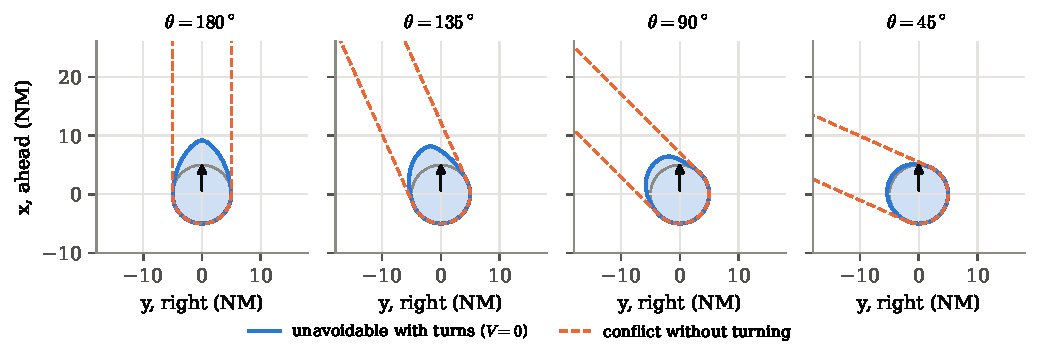
\includegraphics[width=\linewidth]{figs/f5_hj_slices.pdf}
\caption{Slices $\theta=\mathrm{const}$ of the reachability tables ($\Sh=5\NM$, $v_2=v_1=450$\,kt, $T=300$\,s). The
moved aircraft is at the origin heading up (arrow); the other is at $(y,x)$ with track difference $\theta$. Blue: the
states from which no turn avoids the loss; dashed: the conflicts of straight flight; grey: the target disk.}
\label{fig:hj}
\end{figure}

\begin{figure}[t]
\centering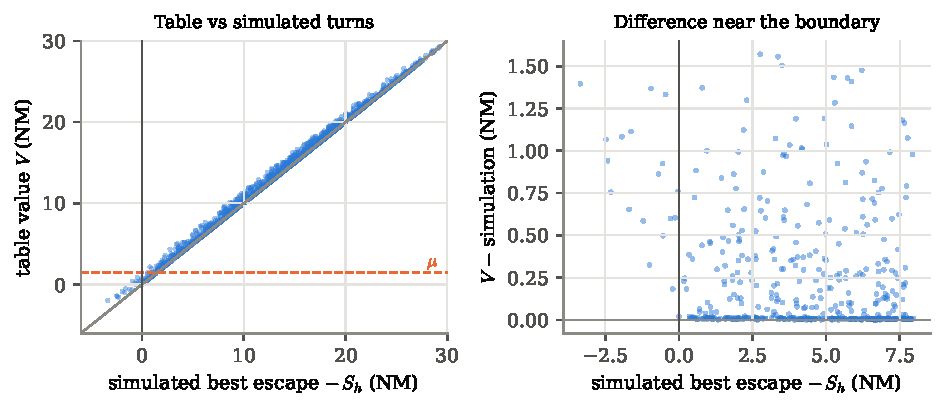
\includegraphics[width=\linewidth]{figs/f6_hj_validation.pdf}
\caption{Validation of the reachability table against simulated turns: the table value against the best simulated
escape (left), and their difference near the boundary (right).}
\label{fig:hjval}
\end{figure}

\subsection{The solver on frozen situations}

On the same situations (\stN\ aircraft each), predicting all trajectories and computing the conflict matrix took a
median of \stMatMed\,ms (at most \stMatMax\,ms); the cost grows with the number of pairs (\cref{fig:stats}, left).
As no one controls these situations, the same encounter appears in several of them until it
becomes a loss: the solver met \stDistinct\ distinct encounters in \stScn\ scenarios, \stConf\ times in all:
\stFut\ times ahead of the encounter, and \stCur\ times already in a loss of separation (no clearance can make $\Phi\ge\Sh+m$ there: the distance is already below the minimum, and the
observation instead gives the levels that separate soonest). It found solutions for \stSolved\ of the \stFut\ future
conflicts (\stSolvedPct\%); the best solution's kind was: \stKinds. The \stUnsolved\ others were close (median time to
infringement \stUnsolvedTf\,s), where only a combination or action on the other traffic remains. A complete solve,
including the rollouts, took a median of \stSolveMed\,s per situation with conflicts (at most \stSolveMax\,s) on a
shared two-core machine. Each rollout of a ten-minute horizon costs about \ROLLval\,s. For the \stConfirmed\
solutions confirmed by rollout, \cref{fig:stats} (right) compares the predicted margin over the minimum with the margin
in the simulation. The simulation is mostly the more favourable --- the prediction keeps every aircraft on its
route while the pilots of the copy also resume, turn and level off as they fly --- and in \stBelowPred\ cases it is
more than half a mile less favourable, at worst by \stWorstGap\NM\ --- more than the margin $m$ covers, which is
why the best solutions are confirmed before they are proposed.

\begin{figure}[t]
\centering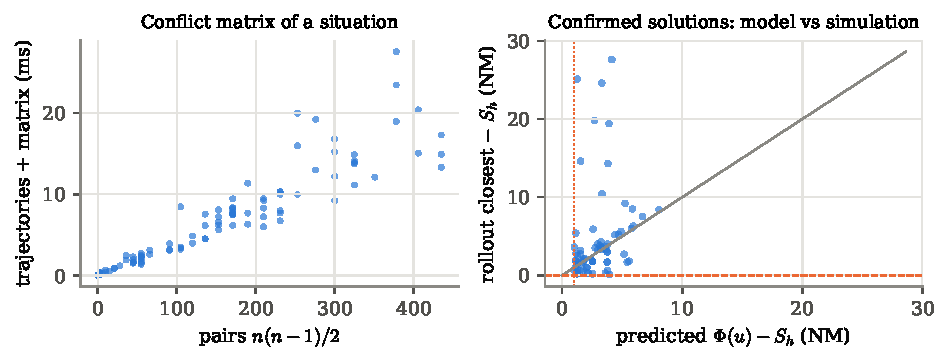
\includegraphics[width=\linewidth]{figs/f7_solver_stats.pdf}
\caption{Left: cost of the trajectory prediction and conflict matrix of a situation against the number of pairs.
Right: for the solutions confirmed by rollout, the margin over $\Sh$ predicted against the margin in the
simulation (dotted: the margin $m$ required of a solution; dashed: the minimum).}
\label{fig:stats}
\end{figure}

\subsection{Closed loop: the solver as a controller}

Finally the solver controlled \clN\ scenarios for 20 simulated minutes each through the AI lab, against the
built-in baseline controller, which assumes, transfers and answers requests the same way but resolves conflicts with
its own rules (speed, then a probed heading, then a level). Both were scored by the lab's evaluation (100 minus
penalties: 25 per loss of separation, 10 per infringement of an active area, track miles, late assumes and
transfers\dots). \Cref{tab:runs} gives the results. Mean score: solver \clSolverMean\ (\clSolverLoss\ losses in
all), baseline \clBaselineMean\ (\clBaselineLoss\ losses). Graded against the solver's solution sets, the baseline's
conflict decisions were: \clBaseGrades\ (the baseline acts on conflicts under eight minutes only, hence the many
conflicts left alone at a given decision).

Neither controller handles the activation of restricted areas (scenario s10) or the non-RVSM aircraft of p05, which
cost both the same penalties; the difference between them is in the losses of separation. The closed loop was also
how two weaknesses of an earlier version of the trajectory model were found. In p06 the solver controller approved a
pilot's request for descent that the radar's probe, with a nominal 2000\,ft/min, found clear; the aircraft, high on
its profile, descended at idle with speedbrakes, at almost twice that, through the level of an aircraft 5\NM\ away,
and was mid-turn after a point. The prediction now flies turns in progress (\cref{sec:traj}) and checks level changes
at the bounds of the rates (\cref{prop:rates}); requests are approved only when both the probe and the solver's check
find them clear.

\begin{table}[t]
\centering\small
\caption{Twenty-minute runs. Score (0--100), losses of separation, clearances given (speed / heading or direct /
level) and the smallest separation in a loss (NM).}
\label{tab:runs}
\setlength{\tabcolsep}{4pt}
\begin{tabular}{l rrcr rrcr}
\toprule
& \multicolumn{4}{c}{Baseline} & \multicolumn{4}{c}{Solver}\\
\cmidrule(lr){2-5}\cmidrule(lr){6-9}
Scenario & score & loss & spd/lat/lvl & min & score & loss & spd/lat/lvl & min\\
\midrule
c01\_cta\_moderate\_wx & 100.0 & 0 & 0/1/0 & -- & 100.0 & 0 & 0/0/0 & -- \\
p01\_ws\_two\_merges & 74.4 & 1 & 0/4/0 & 6.5 & 100.0 & 0 & 0/3/0 & -- \\
p02\_wn\_merges\_and\_climbs & 100.0 & 0 & 0/3/0 & -- & 100.0 & 0 & 9/1/0 & -- \\
p05\_ws\_storms\_arrivals & 95.0 & 0 & 0/0/0 & -- & 95.0 & 0 & 0/0/0 & -- \\
p06\_wn\_capacity\_sequencing & 74.0 & 1 & 0/8/0 & 6.6 & 100.0 & 0 & 0/2/0 & -- \\
s01\_basic\_crossing & 100.0 & 0 & 0/1/0 & -- & 100.0 & 0 & 3/1/0 & -- \\
s02\_climb\_request\_into\_crossing & 100.0 & 0 & 0/0/0 & -- & 100.0 & 0 & 0/0/0 & -- \\
s03\_descent\_through\_opposite & 100.0 & 0 & 0/0/0 & -- & 100.0 & 0 & 0/0/0 & -- \\
s05\_slowdown\_on\_converging\_exit & 100.0 & 0 & 1/1/0 & -- & 100.0 & 0 & 1/0/0 & -- \\
s06\_speed\_up\_into\_crossing & 100.0 & 0 & 3/1/0 & -- & 100.0 & 0 & 1/1/0 & -- \\
s08\_simultaneous\_level\_requests & 100.0 & 0 & 0/0/0 & -- & 100.0 & 0 & 0/0/0 & -- \\
s10\_busy\_mixed & 70.0 & 0 & 7/7/0 & -- & 70.0 & 0 & 1/7/0 & -- \\
\midrule
Mean & 92.8 & 2 & & & 97.1 & 0 & & \\
\bottomrule

\end{tabular}
\end{table}


\section{Discussion and limitations}\label{sec:discussion}

\paragraph{Greedy per conflict.} Each conflict is solved against the predicted trajectories of everyone else, one
at a time. When two conflicts share an aircraft, applying the first solution changes the second; the solver is then
simply run again on the new picture (every five seconds in the panel, at every decision in the AI lab). A joint
formulation --- a mixed-integer programme over the controls of all aircraft with the pairwise CPA as constraints ---
would find solutions this misses, at a cost that grows quickly with the number of aircraft.

\paragraph{Discrete control space.} The super-level set is sampled on a grid of a few dozen controls per
aircraft. The boundary $\{\Phi=\Sh+m\}$ could be located more finely, for instance by bisection along a heading
change or a speed, to propose the smallest sufficient deviation rather than the smallest of the grid.

\paragraph{Model errors.} Trajectories assume the present wind along the path, constant speeds between changes and
nominal vertical rates; other controllers' intentions are unknown. The margin $m$, the confirmation by rollout and
the re-solve at every update address these, but the solution set is only as good as the prediction of the
others. The Hamilton--Jacobi table is computed for a single nominal speed of the moved aircraft and five speed
ratios, without wind, and is first-order accurate.

\paragraph{What the solver does not see.} Restricted areas that become active, weather cells and the non-RVSM
status of an aircraft enter the solution set only through the pilot's own check of a clearance, not as constraints
of their own; the solver does not plan a route around an area or a cell. Scenario s10 shows the cost: both
controllers incurred three area infringements.

\paragraph{Costs.} The weights of $J$ encode the unit's order of preference and priority rule; they are hand-set.
Recorded controller decisions --- from the solo radar and the exercises --- could be used to fit them, the solution
set providing the alternatives against which each human choice is compared.

\section{Conclusion}

Exact CPA on piecewise-linear trajectories turns conflict detection into a matrix computation and makes the quality
of any candidate clearance a single number, $\Phi(u)$, the closest it brings the aircraft to anyone. The solution set
is the region of the control space where that number clears the minimum with a margin, ranked by the controller's
conventions, filtered at close range by reachability, and confirmed by simulation. It serves the trainee as advice,
a language model as guidance and grading, and the simulator as a controller of reference.

\begin{thebibliography}{99}\small
\bibitem{kuchar2000} J.~K.~Kuchar and L.~C.~Yang. A review of conflict detection and resolution modeling methods.
\emph{IEEE Transactions on Intelligent Transportation Systems}, 1(4):179--189, 2000.
\bibitem{fiorini1998} P.~Fiorini and Z.~Shiller. Motion planning in dynamic environments using velocity obstacles.
\emph{International Journal of Robotics Research}, 17(7):760--772, 1998.
\bibitem{hoekstra2002} J.~M.~Hoekstra, R.~N.~H.~W.~van Gent and R.~C.~J.~Ruigrok. Designing for safety: the
`free flight' air traffic management concept. \emph{Reliability Engineering \& System Safety}, 75(2):215--232, 2002.
\bibitem{pallottino2002} L.~Pallottino, E.~M.~Feron and A.~Bicchi. Conflict resolution problems for air traffic
management systems solved with mixed integer programming. \emph{IEEE Transactions on Intelligent Transportation
Systems}, 3(1):3--11, 2002.
\bibitem{durand1996} N.~Durand, J.-M.~Alliot and J.~Noailles. Automatic aircraft conflict resolution using genetic
algorithms. In \emph{Proceedings of the ACM Symposium on Applied Computing}, 1996.
\bibitem{mitchell2005} I.~M.~Mitchell, A.~M.~Bayen and C.~J.~Tomlin. A time-dependent Hamilton--Jacobi formulation of
reachable sets for continuous dynamic games. \emph{IEEE Transactions on Automatic Control}, 50(7):947--957, 2005.
\bibitem{tomlin1998} C.~Tomlin, G.~J.~Pappas and S.~Sastry. Conflict resolution for air traffic management: a study in
multiagent hybrid systems. \emph{IEEE Transactions on Automatic Control}, 43(4):509--521, 1998.
\bibitem{osher2003} S.~Osher and R.~Fedkiw. \emph{Level Set Methods and Dynamic Implicit Surfaces}. Springer, 2003.
\bibitem{crandall1983} M.~G.~Crandall and P.-L.~Lions. Viscosity solutions of Hamilton--Jacobi equations.
\emph{Transactions of the American Mathematical Society}, 277(1):1--42, 1983.
\end{thebibliography}

\appendix
\section{Parameters}\label{app:params}
\begin{center}
\small
\begin{tabular}{lll}
\toprule
Symbol & Value & Meaning \\
\midrule
$H$ & 600 s & prediction horizon of the solver\\
$m$ & 1.0 NM & margin on $\Sh$ for a solution\\
$\delta_s$ & 40 s & time to achieve a speed change\\
$\delta_p$ & 6 s & pilot delay\\
$\omega$ & $3^\circ$/s & standard-rate turn\\
$\tau$ & 120, 240, 360 s & durations of a delaying vector\\
$\varepsilon$ & 0.3 & cost tolerance of the optimal set\\
$T_{\mathrm{HJ}}$ & 300 s & horizon of the reachability tables\\
$\mu$ & 1.5 NM & threshold on $V$ (``a turn is enough'')\\
grid & $101\times101\times60$ & $[-45,45]^2$ NM $\times\ [0,2\pi)$\\
$k$ & 2 & solutions confirmed by rollout per conflict\\
\bottomrule
\end{tabular}
\end{center}

\end{document}
